\documentclass[12pt,twoside,a4paper]{article} 

\usepackage{color,amssymb,amsmath,mathtools} 
\usepackage{fullpage,caption, listings,clrscode,placeins}
\usepackage{amsmath,bm}
\usepackage{subfig}
\usepackage{float}
\usepackage{algorithm}
\usepackage{algpseudocode}
% \usepackage{graphicx}
 
 % Metadata info
\newcommand{\mytitle}{Project 2} 
\newcommand{\mydate}{\today}
\newcommand{\myauthors}{Prameth Gaddale (pqg5273@psu.edu)}

% Setting Hyperref parameters
\usepackage[
	bookmarks,
	bookmarksnumbered,
	pdfpagemode={UseOutlines},
	plainpages=false,
	pdfpagelabels=true,
	pdfauthor={\myauthors},
	pdftitle={\mytitle},
	pagebackref=true,
	pdftex,
	colorlinks=true,
	linkcolor=red,
	urlcolor={blue}, 
	pagebackref=true]
	{hyperref}

\title{\mytitle}
\author{\myauthors}
\date{\mydate}

% Some useful commands from CVPR
\usepackage{xspace}
\makeatletter
\DeclareRobustCommand\onedot{\futurelet\@let@token\@onedot}
\def\@onedot{\ifx\@let@token.\else.\null\fi\xspace}
\def\eg{\emph{e.g}\onedot} \def\Eg{\emph{E.g}\onedot}
\def\ie{\emph{i.e}\onedot} \def\Ie{\emph{I.e}\onedot}
\def\cf{\emph{c.f}\onedot} \def\Cf{\emph{C.f}\onedot}
\def\etc{\emph{etc}\onedot} \def\vs{\emph{vs}\onedot}
\def\wrt{w.r.t\onedot} \def\dof{d.o.f\onedot}
\def\etal{\emph{et~al}\onedot}
\makeatother


\pagestyle{empty}
\usepackage{fancyref,fancyhdr}
%\usepackage[hmarginratio=1:1, top=2.0cm, bottom=5.0cm, left=1cm, right=1cm]{geometry}
\setlength{\headheight}{14pt}
\setlength{\headsep}{15pt}
\setlength{\footskip}{50pt}
\pagestyle{fancy}
\fancyhf{}
\fancyhf[HLE,HRO]{\footnotesize{\myauthors}}
\fancyhf[HLO,HRE]{\footnotesize{\mydate}}
\fancyhf[FLO,FRE]{\footnotesize{\mytitle}} 
\fancyhf[FLE,FRO]{\thepage }


\usepackage[pdftex]{graphicx}
\DeclareGraphicsExtensions{.pdf,.png,.jpg,.eps}

% 
\usepackage[numbers, sort&compress]{natbib}

\usepackage[senames,dvipsnames,svgnames,table]{xcolor}

\newenvironment{tightitemize} % Defines the tightitemize environment which modifies the itemize environment to be more compact
{\vspace{-\topsep}\begin{itemize}\itemsep1pt \parskip0pt \parsep0pt}
{\end{itemize}\vspace{-\topsep}} 

% If you want to write proofs
\newtheorem{claim}{Claim}[section]
\newtheorem{lemma}{Lemma}[section]

% Some useful packages (look at booktabs for good looking tables)
\usepackage{subcaption,booktabs,placeins}

%BEGIN THE DOCUMENT

\begin{document}
\maketitle

\begin{abstract}

This project primarily deals with feature subset selection for the classification problem through the use of the Taiji sequence dataset. The use of feature selection is to solve the issues of 'Curse of Dimensionality', computational efficiency, easier data collection, storage size, and interpretability through the strategy of dimensionality reduction. Implementations of the feature selection algorithms in this project include \textbf{Filtering} and \textbf{Wrapper} methods. 

\end{abstract}
\vspace{1ex}

\tableofcontents
\pagebreak
% SECTIONS
\section{Introduction}
The last project followed an approached where vanilla classification problem was implemented through the use of \textit{Fisher Linear Discriminant Analysis}, which would not necessarily correspond to complexity involved by higher number of feature dimensions \cite{ChrisPRML}.

The approach previously taken in the \textit{Project-1} didn't involve any data normalization or feature engineering steps which are essential pre-processing steps for the data to be involved with before being used for making crucial classification decisions/predictions.

\textit{Feature Selection} which is the part of the family of \textit{Feature Engineering} methods which involve the steps followed before fitting the training the final regression or classification model to improve the performance through the use of relevant features. Modern machine learning datasets contain thousands of features corresponding to the dataset used. 

However, each of them correspond to either useful/useless category of features used for training the parameters of the machine learning model. For example, in the given dataset there are features that don't have any variance, or have a constant value for all the training examples. It would be wise to exclude the feature in that case to gain more leverage in overall computational efficiency, storage and algorithmic efficiency.
%-------------------------------------------------------------------------
\section{Approach}

\textit{Feature Selection} in a broad way consists of choosing a proper subset of features of all the given features based on some defined criterion. Feature Selection operations performed in this project involve the use of:
\begin{itemize}
    \item Filter Method
    \item Wrapper Method
\end{itemize}
Both of the methods differ based upon the optimization criterion set by the objective function.

\textit{Filter Methods} select the best features based on their discrimination potential through the use of a chosen metric. There is no actually iterative optimization taking place in this algorithms, however, the features are selected based of metric ranking. 

On the other hand, \textit{Wrapper Methods} select the best feature subset through a criteria set by solving a classification task on the subset iteratively through a search algorithm.

\begin{figure}
    \centering
    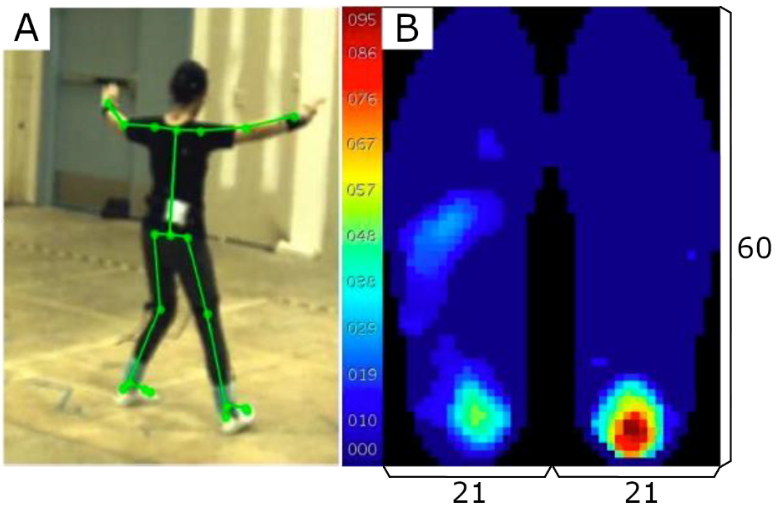
\includegraphics[width=0.7\linewidth]{data.png}
    \caption{PSU-TMM100 Dataset (A). The Video Data with 17 joints. (B). The left-right foot pressure sensor heatmap.}
    \label{fig: DATA}
\end{figure}

\subsection{Data}

The given dataset is PSU-TMM100 (Taiji) based on human-sequence forms, rendered using 3D motion capture devices from various crucial body parts and foot pressure sensors. 

The 3D body joints from MoCAP captures 17 joints and the foot pressure data consists 1910 elements as shown in \ref{fig: DATA}. The total number of features come out to be 1961 for each observation.
\subsubsection*{Data Splitting Strategy}
The training process involves the \textit{Leave One Subject Out} strategy during classification to enable testing with pseudo-unseen data and resembles the prediction based off in a real scene setting. 

%-------------------------------------------------------------------------
\subsection{Filter Method}

Feature selection filtering is a technique used to select a relevant subset of features from a larger given set of features. In a way, reducing the use of irrelevant and redundant features in the given data. The reduced redundancy has help find gains in the efficiency of the overall classification process. The goal of feature selection is to improve the model performance and reduce the risk of over-fitting \cite{statistical}.

Filter methods usually evaluate each of the given feature independently and assign a corresponding score to that feature based on its relevance to the target vector. Features that score below a certain threshold are then removed from consideration, or can be sorted out by taking a set of features from thr top. The commonly used filter methods include:

\begin{itemize}
    \item Variance Ratio
    \item Augmented Variance Ratio
    \item Minimum Redundancy Maximum Relevance
\end{itemize}

The metric implemented in this \textit{Report} is the \textit{Variance Ratio} which is defined as in \eqref{1}

\begin{equation}\label{1}
    VR(F) = \frac{Var(S_F)}{\frac{1}{C}\sum_{k = 1,...,C} Var_k(S_k)}
\end{equation}

\begin{itemize}
    \item $VR(F)$ : Variance Ratio Score for the Feature $F$
    \item $Var(S_F)$: Within class variance
    \item $Var_k(S_F)$: Within class variance of the class \textit{k}
    \item $C$: Total number of classes.
\end{itemize}

Filter approaches are generally easy to implement and computationally efficient, making them a popular choice for feature selection in large data sets. We represent the variance ratio for a particular feature to be the ratio of the inter class variance contained in that feature to the ratio of the mean of the intra class variances for all the classes. Therefore, a larger value of the variance ratio would indicate a more desirable feature with the highest variance ratio feature being the most desirable one. \\

\subsubsection*{Filter Method Algorithm}
The algorithm of the Filter Method is given by,
\begin{itemize}
    \item Consider all the given features, $F$ in the Train set.
    \item Ensuring the filter feature count, $filter\_feature\_count$ to be less than total dimensions, start iterating over all the features.
    \item Compute the variance, $Var(F)$ of each feature, and compute the ratio with the help of per-class variance $Var_k(S_F)$.
    \item Receive the indices by sorting the variance scores computed from the previous step.
    \item Hence, we can get the top-100 features from the sorted list indices which represent the filtering method features.
\end{itemize}

%-------------------------------------------------------------------------
\subsection{Wrapper Method}

Wrapper methods typically employ a search algorithm to select a subset of features based on their impact on model performance. Unlike filter methods, which evaluate features independently, wrapper methods considers the interdependence between the features and the model.

Generally the wrapper methodology involves defining the target vector and a set of potential features (predictors). Upon that, we'd define a search algorithm procedure that iteratively adds or removes features to/from the model. Subsequently, a machine learning model is trained using a subset of features and the performance of the model is evaluated either through the use of training data or validation data. Consequently, we use the performance metric to guide the search algorithm in selecting the best subset of features. Upon finding a good enough set of features from the search procedure, we train a classification model using the selected subset of features.

\subsubsection*{Optimization Criterion}
    

\subsubsection*{Wrapper Method Algorithm}
The algorithm of the Wrapper method through the use of Sequential Forward Selection is given by,
\begin{itemize}
    \item Initially, consider an empty set of the features, and store the complete set of features.
\end{itemize}

%-------------------------------------------------------------------------
\section{Report}

%-------------------------------------------------------------------------
\subsection{Model Pipeline}
\begin{itemize}
    \item The given data was first normalized with respect to the minimum and maximum values in the design matrix. Hence, the range is normalized to be [0,1].
    \item After the data normalization part, the number of features from the filter method is specified and the filtering method is run with the criterion of Variance Ratio.
    \item In our case, we pass all the 1961 features and receive the 100 selected features sorted based on the variance score and their associated corresponding variance scores.
    \item Upon receiving the filtered features, we implement the wrapper method with sequential forward selection algorithm for searching the relevant features based on the classification accuracy on the linear discriminant classifier.
    \item Then the features received from the wrapper method are used to train a K-Nearest Neighbor classifier with $k=10$.
\end{itemize}

The schematic of the model pipeline is shown in .

\begin{figure}[H]
    \centering
    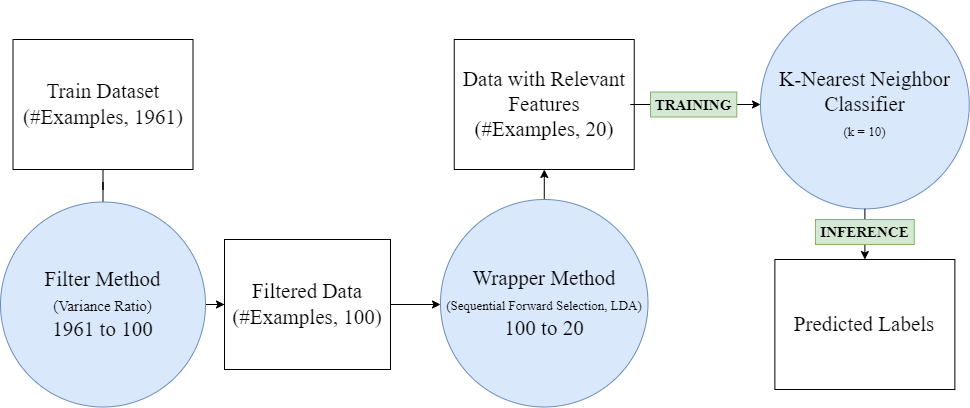
\includegraphics[width=0.7\linewidth]{pipeline.png}
    \caption{Model Pipeline}
    \label{fig: NFW1}
\end{figure}

\pagebreak
%-------------------------------------------------------------------------
\subsection{Classification Results}

%-------------------------------------------------------------------------
\subsubsection{Baseline Model (No Filter, No Wrapper)}
As a baseline measure for comparison purposes, a model without feature selection of filtering and wrapping methodology was implemented. The data used for the classification involved the use of all the $1961$ features for train and test phases. The classification model used for training and inference was \textit{K-Nearest Neighbors Classifier} from \textit{Scikit-Learn} with $k=10$.

\subsubsection*{Classification Rates}
The classification model is not generalizing well over the test set as being trained on the wide variety of features. Its evident from the figures of the per class training and test set accuracies.
\begin{figure}[H]
    \centering
    \includegraphics[width=0.8\linewidth]{nfnw/overall_per_class_train.png}
    \caption{Training Set Confusion Matrix: No Filter, No Wrapper}
    \label{fig: NFW1}
\end{figure}

\begin{figure}[H]
    \centering
    \includegraphics[width=0.8\linewidth]{nfnw/overall_per_class_test.png}
    \caption{Test Set Confusion Matrix: No Filter, No Wrapper}
    \label{fig: NFW2}
\end{figure}


\begin{table}[H]
\centering
\begin{tabular}{|l|l|l|}
\hline
\multicolumn{1}{|c|}{\textbf{Category}} & \multicolumn{1}{c|}{\textbf{Train}} & \multicolumn{1}{c|}{\textbf{Test}} \\ \hline
\textbf{Subject 1}  & 0.927 & 0.617 \\ \hline
\textbf{Subject 2}  & 0.929 & 0.585 \\ \hline
\textbf{Subject 3}  & 0.930 & 0.624 \\ \hline
\textbf{Subject 4}  & 0.928 & 0.610 \\ \hline
\textbf{Subject 5}  & 0.928 & 0.640 \\ \hline
\textbf{Subject 6}  & 0.926 & 0.657 \\ \hline
\textbf{Subject 7}  & 0.927 & 0.669 \\ \hline
\textbf{Subject 8}  & 0.929 & 0.665 \\ \hline
\textbf{Subject 9}  & 0.929 & 0.683 \\ \hline
\textbf{Subject 10} & 0.929 & 0.543 \\ \hline
\textbf{Overall}    & 0.928 & 0.623 \\ \hline
\end{tabular}
\caption{Subject-wise accuracy rates for no filter with no wrapper configuration.}
\label{tab:NFNWT}
\end{table}

The table and the subject-wise accuracies represent the classic case of over-fitting, as the test set accuracy is far below the training set accuracy.

\begin{figure}[H]
    \centering
    \includegraphics[width=1.0\linewidth]{nfnw/subject_wise_acc.png}
    \caption{Subject-wise training and testing accuracies.}
    \label{fig: NFW3}
\end{figure}

\subsubsection*{Confusion Matrix}

\begin{figure}[H]
    \centering
    \includegraphics[width=0.5\linewidth]{nfnw/overall_train_conf_mat.png}
    \caption{Training Set Confusion Matrix: No Filter, No Wrapper}
    \label{fig: NFW4}
\end{figure}

\begin{figure}[H]
    \centering
    \includegraphics[width=0.5\linewidth]{nfnw/overall_test_conf_mat.png}
    \caption{Test Set Confusion Matrix: No Filter, No Wrapper}
    \label{fig: NFW5}
\end{figure}

In this case, its observed that there is a high degree of mis-classification rate in the features close to each other, as indicated by the darker shades in near-diagonal
elements.

That would give us the reasoning behind the poses which might not be all that different from each other. They may have a number of joints positioned in similar ways without substantial change in the feet movement being likely explanations to be the cause of this over-fitting behavior.

This behavior justifies the performance of the feature selection methods because we now recognize the need to select those joints or the associated feet pixels which can potentially vary significantly, or be discriminative enough for even these same poses. Hopefully, adding the filter would help curb the over-fitting nature of the KNN Classifier employed.

%-------------------------------------------------------------------------
\subsubsection{Filter, No Wrapper}

The filtering method with Variance Ratio was implemented and the top 100 features were considered. The processed training data was used to fit the \textit{K-Nearest Neighbors Classifier} from \textit{Scikit-Learn} with $k=10$.

\subsubsection*{Classification Rates}
Let us look at the classification rates for the features both for training and test data followed by the the training and testing classification rates per subject as shown in the following figures.

\begin{figure}[H]
    \centering
    \includegraphics[width=0.7\linewidth]{fnw/overall_per_class_train.png}
    \caption{Per Class Training Accuracy per Form}
    \label{fig: F1}
\end{figure}

\begin{figure}[H]
    \centering
    \includegraphics[width=0.7\linewidth]{fnw/overall_per_class_test.png}
    \caption{Per Class Testing Accuracy per Form}
    \label{fig: F2}
\end{figure}

Clearly, there is a minor improvement observed in the test classification rates. This comes at the expense of training classification rates which would always increase as long as we gave it more features, associating this problem with a tradeoff with features and training accuracy. However, the over-fitting problem has ameliorated at a certain extent with nearly all features reaching more than 40\% test accuracy with some noticeable outliers.

\begin{table}[H]
\centering
\begin{tabular}{|l|l|l|}
\hline
\multicolumn{1}{|c|}{\textbf{Category}} & \multicolumn{1}{c|}{\textbf{Train}} & \multicolumn{1}{c|}{\textbf{Test}} \\ \hline
\textbf{Subject 1}  & 0.924 & 0.664 \\ \hline
\textbf{Subject 2}  & 0.934 & 0.666 \\ \hline
\textbf{Subject 3}  & 0.935 & 0.722 \\ \hline
\textbf{Subject 4}  & 0.935 & 0.776 \\ \hline
\textbf{Subject 5}  & 0.937 & 0.774 \\ \hline
\textbf{Subject 6}  & 0.935 & 0.767 \\ \hline
\textbf{Subject 7}  & 0.937 & 0.782 \\ \hline
\textbf{Subject 8}  & 0.935 & 0.779 \\ \hline
\textbf{Subject 9}  & 0.929 & 0.642 \\ \hline
\textbf{Subject 10} & 0.938 & 0.685 \\ \hline
\textbf{Overall}    & 0.934 & 0.726 \\ \hline
\end{tabular}
\caption{Subject-wise accuracy rates for filter with no wrapper.}
\label{tab:FNWT}
\end{table}

Its evident from \ref{tab:FNWT} that the model is overfitting the training data distribution as the training accuracy rate is substantially higher compared to the testing accuracy rate.

\begin{figure}[H]
    \centering
    \includegraphics[width=0.8\linewidth]{fnw/subject_wise_acc.png}
    \caption{Subject-wise training and testing accuracies.}
    \label{fig: F3}
\end{figure}

Looking at the subject-wise training and test accuracies for each individual subjects, we find that nearly all subjects reach more than 60\% test accuracy. Hence, which is much better than the no filter method, however there is constant steady behavior expected with the training accuracy.

\subsubsection*{Confusion Matrix}

Looking at the confusion matrices, its evident that the over-fitting issue hasn't been solved yet. The training set confusion matrix diagonal elements are bright compared to the rest which is the desirable feature. \\
However, the testing set confusion matrix hasn't been set yet. Hopefully introducing a wrapper method suitable to the data would be helpful in fixing the issue.

\begin{figure}[H]
    \centering
    \includegraphics[width=0.5\linewidth]{fnw/overall_train_conf_mat.png}
    \caption{Training Set Confusion Matrix: Filter, No Wrapper}
    \label{fig: F4}
\end{figure}

\begin{figure}[H]
    \centering
    \includegraphics[width=0.5\linewidth]{fnw/overall_test_conf_mat.png}
    \caption{Test Set Confusion Matrix: Filter, No Wrapper}
    \label{fig: F5}
\end{figure}

%-------------------------------------------------------------------------
\subsubsection{Filter, Wrapper}

The filtering method with Variance Ratio as the measure was implemented. The top 100 features passed through the wrapper method with Sequential Forward Selection. The processed training data was used to fit the \textit{K-Nearest Neighbors Classifier} from \textit{Scikit-Learn} with $k=10$.

\subsubsection*{Classification Rates}

\begin{figure}[H]
    \centering
    \includegraphics[width=0.7\linewidth]{results/overall_per_class_train.png}
    \caption{Per Class Training Accuracy per Form}
    \label{fig: FW1}
\end{figure}

\begin{figure}[H]
    \centering
    \includegraphics[width=0.7\linewidth]{results/overall_per_class_test.png}
    \caption{Per Class Testing Accuracy per Form}
    \label{fig: FW2}
\end{figure}

\begin{figure}[H]
    \centering
    \includegraphics[width=0.7\linewidth]{results/subject_wise_acc.png}
    \caption{Subject-wise training and testing accuracies.}
    \label{fig: FW3}
\end{figure}

\begin{table}[H]
\centering
\begin{tabular}{|l|l|l|}
\hline
\multicolumn{1}{|c|}{\textbf{Category}} & \multicolumn{1}{c|}{\textbf{Train}} & \multicolumn{1}{c|}{\textbf{Test}} \\ \hline
\textbf{Subject 1}  & 0.924 & 0.664 \\ \hline
\textbf{Subject 2}  & 0.934 & 0.666 \\ \hline
\textbf{Subject 3}  & 0.935 & 0.722 \\ \hline
\textbf{Subject 4}  & 0.935 & 0.776 \\ \hline
\textbf{Subject 5}  & 0.937 & 0.774 \\ \hline
\textbf{Subject 6}  & 0.935 & 0.767 \\ \hline
\textbf{Subject 7}  & 0.937 & 0.782 \\ \hline
\textbf{Subject 8}  & 0.935 & 0.779 \\ \hline
\textbf{Subject 9}  & 0.929 & 0.642 \\ \hline
\textbf{Subject 10} & 0.938 & 0.685 \\ \hline
\textbf{Overall}    & 0.934 & 0.726 \\ \hline
\end{tabular}
\caption{Subject-wise accuracy rates for filter and wrapper method.}
\label{tab:FNWT}
\end{table}

\subsubsection*{Confusion Matrix}

\begin{figure}[H]
    \centering
    \includegraphics[width=0.5\linewidth]{results/overall_train_conf_mat.png}
    \caption{Training Set Confusion Matrix: Filter and Wrapper}
    \label{fig: FW4}
\end{figure}

\begin{figure}[H]
    \centering
    \includegraphics[width=0.5\linewidth]{results/overall_test_conf_mat.png}
    \caption{Test Set Confusion Matrix: Filter and Wrapper}
    \label{fig: FW5}
\end{figure}

\subsubsection*{Most Discriminative Features: Filter}

\begin{figure}[H]
    \centering
    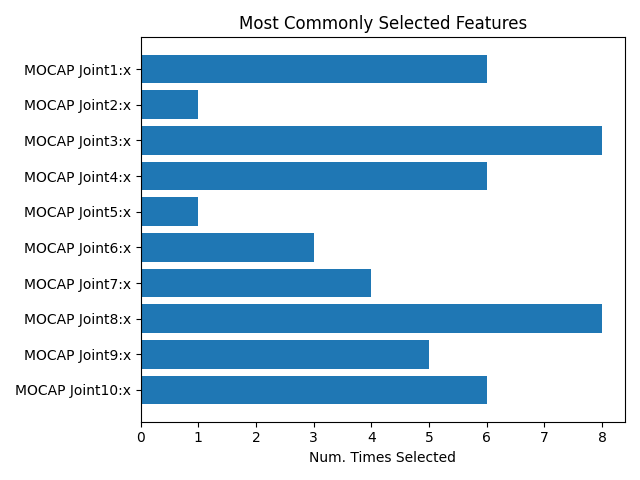
\includegraphics[width=0.7\linewidth]{results/selected_feats.png}
    \caption{Most Discriminative Features: Filter}
    \label{fig: FW6}
\end{figure}

\subsubsection*{Most Commonly Selected Features: Wrapper}

\begin{figure}[H]
    \centering
    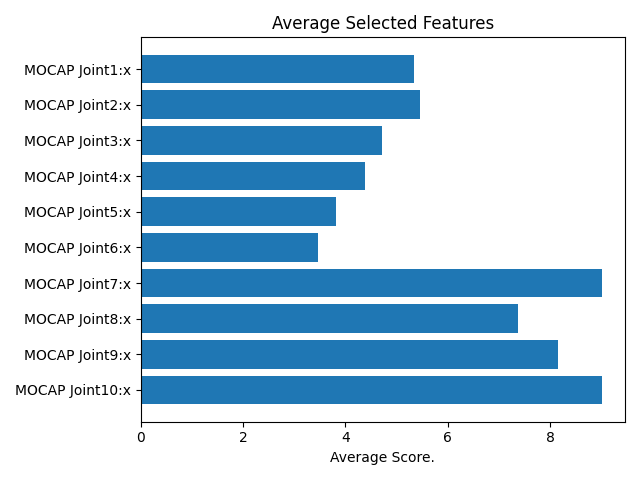
\includegraphics[width=0.7\linewidth]{results/avg_filter_scores.png}
    \caption{Most Commonly Selected Features: Wrapper}
    \label{fig: FW7}
\end{figure}

%-------------------------------------------------------------------------
\subsection{Question: Dataset Size Sufficiency}

%-------------------------------------------------------------------------
\section{Conclusion}

%-------------------------------------------------------------------------
\section{Extra Credit}
Here are my solutions for the \textbf{Extra Credit} section.
\subsection{Ensemble Learning}

%-------------------------------------------------------------------------

% BIBLIOGRAPHY
{\small
\bibliographystyle{IEEEtranN}
\bibliography{mybib}}

\end{document}
